This question refers to Figure~\ref{fig:basic_rnn}. Give an example of a domain or problem where the following types of RNN architectures could be used: (2 points each)
\begin{itemize}
        \item Figure 1b: many to one.
        \item Figure 1c: one to many
        \item Figure 1d: many in, then many out.
        \item  Figure 1e: Simultaneous many in, many out.
 \end{itemize}
  \begin{figure}[h]
\centering

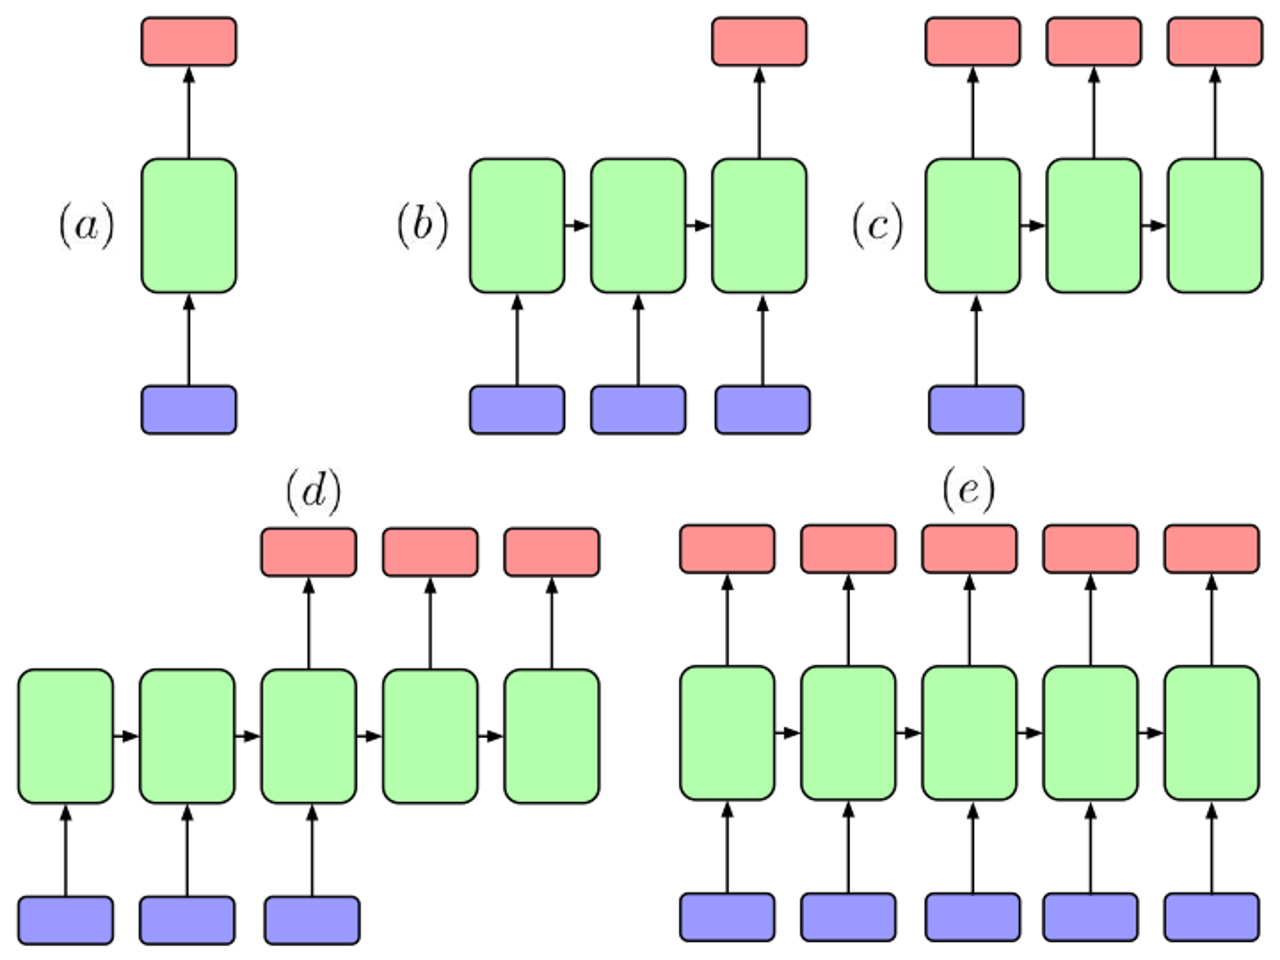
\includegraphics[width=0.5\linewidth]{images/rnn.png}

\caption{Basic Recurrent Network Architectures (except (a), which is feedforward!)}\label{fig:basic_rnn}
\end{figure}

\begin{tcolorbox}

\begin{enumerate}[label=(\alph*)]
        \item  (a excluded)
        \item Determining the sentiment of an article (many words to one sentiment)
        \item Captioning an image (one image to many words)
        \item Translating chinese to english (many words to many words)
        \item Generating subtitles for a video (frames at many points to captions at those same points)
\end{enumerate}

\end{tcolorbox}
